\documentclass{article}
\usepackage[margin=1in]{geometry}
\usepackage{graphicx}
\usepackage[fleqn]{amsmath}
\usepackage{color}
\usepackage{lipsum}
\begin{document}
\setcounter{totalnumber}{5}
   \begin{flushright}
      \Large\textbf{Steven Murr}\\
      \large\textit{HW 3.2}\\
      \large\textit{Problems = \{ 1abc, 2abc, 3, 10, 21, 22, 23, 24, 25ab, 26ab \}} \\
   \end{flushright}
\begin{flushleft}
\makeatletter% Set distance from top of page to first float
\setlength{\@fptop}{5pt}
\makeatother
\setlength\parindent{0pt}1) Determine whether each of these functions is $O(x)$ \\
\setlength\parindent{24pt}a) $f(x) = 10$ \\
\setlength\parindent{48pt} $x > 10$ whenever $x > 10$\\
\setlength\parindent{48pt} We then replace 10 with x and get $x \leq c*x$ \\
\setlength\parindent{48pt} Thus, f(x) is O(x) for $C = 10, k = 1$\\
\setlength\parindent{24pt}b) $3x + 7$ \\
\setlength\parindent{48pt} Since $x > 7$ whenever $x > 7$ we can replace 7 with x. \\
\setlength\parindent{48pt} $3x + x \leq 4x$ \\
\setlength\parindent{48pt} This yields $4x \leq c*x$ \\
\setlength\parindent{48pt} Thus, f(x) is O(x) when C = 4, k = 7 \\
\setlength\parindent{24pt}c) We know that a function is O(x) of it's largest exponent.  Since $x^2 + x + 1$ has an $x^2$ we know \\that this is not O(x).  It's in fact $O(x^2)$. \\
~\\
\setlength\parindent{0pt}2) Determine whether each of these functions is $O(x^2)$ \\
\setlength\parindent{24pt}a) $f(x) = 17x + 11$ \\
\setlength\parindent{48pt} Since $x^2 > 11$ whenever $x^2 > 11$ we can write the equation as $17x^2 + x^2$ which becomes $18x^2$.  \\
\setlength\parindent{48pt} Thus, f(x) is $O(x^2)$ when C = 18, k = 11 \\
\setlength\parindent{24pt}b) $f(x) = x^2 + 1000$ \\
\setlength\parindent{48pt} Since we know that $x^2 > 1000$ whenever $x^2 > 1000$ thus we can replace 1000 with $x^2$.\\
\setlength\parindent{48pt} $x^2 + x^2 \leq 2x^2$\\
\setlength\parindent{48pt} Thus, f(x) is O(x) whenever $C = 2, k = \sqrt{1000}$ \\
\setlength\parindent{24pt}c) $f(x) = x logx$ \\
\setlength\parindent{48pt} Since $x log x \leq x^2$ for all values of x C = 1, k = 0.\\

~\\
\setlength\parindent{0pt}3) Use the definition of "f(x) is O(g(x))" to show that $x^4 + 9x^3 + 4x + 7 is O(x^4)$ \\
\setlength\parindent{24pt} We first append $x^4$ to each of the exponents like: \\
\setlength\parindent{24pt}$x^4 + x^4 + x^4 + x^4 = 4x^4$.  C = 4, k = 9 \\
~\\

\setlength\parindent{0pt}10) Show that $x^3 is O(x^4)$ but that $x^4$ is not $O(x^3)$ \\
\setlength\parindent{24pt} The definition for Big-O notation is $| f(x) | \leq C | g(x) |$ \\
\setlength\parindent{48pt} $x^3$ is $O(x^4)$ \\
\setlength\parindent{48pt} $x^3 \leq x^4$ however $x^4$ is not $\leq x^3$ therefore a larger exponent cannot be Big-O of a \\smaller exponent. \\
~\\
\setlength\parindent{0pt}21) Arrange the functions $\sqrt{n}, 1000logn, nlogn, 2n!, 2^n, 3^n$ and $n^2 / 1,000,000$ in a list so that each function is big-O of the next function. \\
\setlength\parindent{24pt} $\frac{n^2}{1,000,000} > \sqrt{n} > xlog(x) > 2^x > 2x! > 3^x > 1000log(x) $ \\
\setlength\parindent{0pt}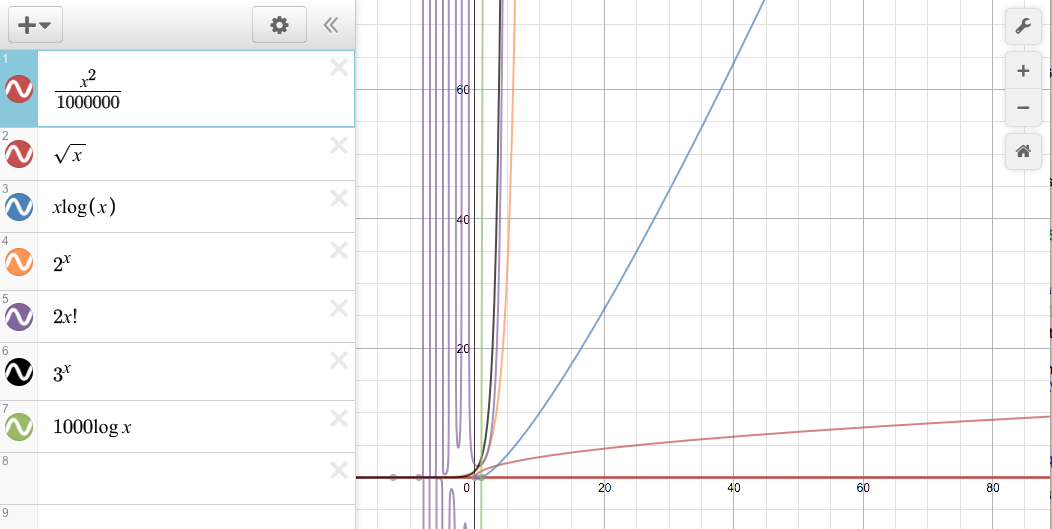
\includegraphics[width=\textwidth]{graph.png} \\
~\\
\setlength\parindent{0pt}22) Arrange the functions $(1.5)^n, n^{100}, (long)^3, \sqrt{n}logn, 10^n, (n!)^2, $ and $n^{99} + n^{98}$ in a list so that each function is big-O of the next function. \\
\setlength\parindent{24pt} $(logx)^3 > \sqrt{x} log x > (1.5)^x > (x!)^2 > 10^x > x^{99} + x^{98} > x^{100}$ \\
~\\
\setlength\parindent{0pt}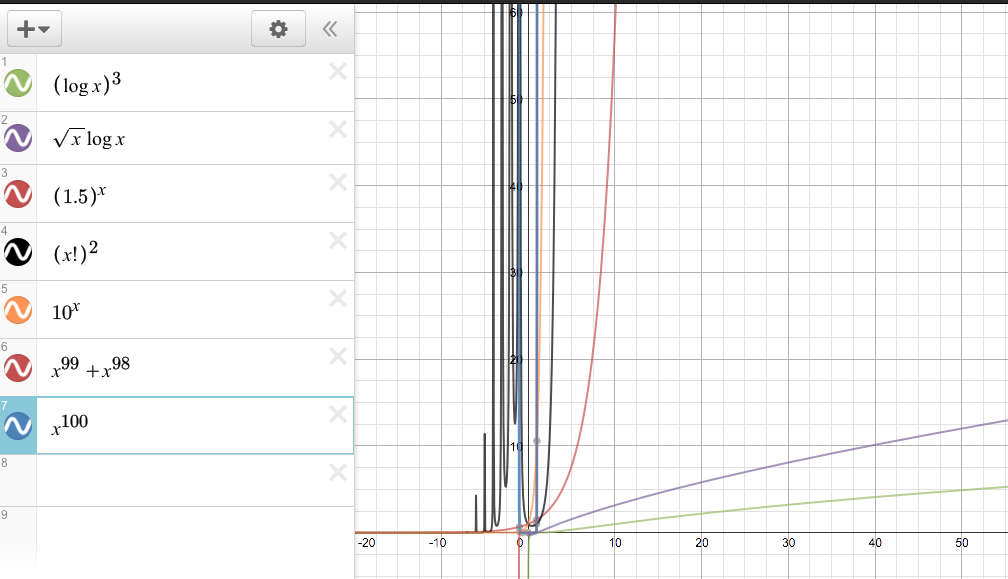
\includegraphics[width=\textwidth]{graph2.png} \\
~\\
\setlength\parindent{0pt}23) Suppose that you have two different algorithms for solving a problem.  To solve a problem of size n, the first algorithm uses exactly n(log n) operations and the second algorithm uses exact $n^{\frac{3}{2}}$ operations.  As n grows, which algorithm uses fewer operations? \\
\setlength\parindent{24pt} Exponential operations require more operations than logarithmic ones.  n(log n) uses fewer operations. \\
~\\
\setlength\parindent{0pt}25)Give as good a big-O estimate as possible for each of these functions. \\
\setlength\parindent{24pt}a) $(n^2 + 8)(n + 1)$ \\
\setlength\parindent{48pt} $n^3 + n^2 + 8n + 8$ \\ 
\setlength\parindent{48pt} Algorithms are big-O of it's highest exponent.  This algorithm is $O(x^3)$ \\
\setlength\parindent{24pt}b) $(n log n + n^2)(n^3 + 2)$\\
\setlength\parindent{48pt} $n^3 logn + 2logn + n^5 + 2n^2$ \\
\setlength\parindent{48pt} $n^5$ is the largest value so, $O(n^5)$\\
\setlength\parindent{24pt}c) $(n! + 2^n)(n^3 + log(n^2 + 1))$\\
\setlength\parindent{48pt}$n!n^3$ \\
~\\
\setlength\parindent{0pt}26) Give a big-O estimate for each of these functions.  For the function $g$ in your estimate $f(x)$ is $O(g(x))$, use a simple function $g$ of smallest order. \\
\setlength\parindent{24pt}a) $(n^3 + n^2logn)(logn + 1) + (17logn+19)(n^3 + 2)$ \\
\setlength\parindent{48pt} $O(n^3)$ \\
\setlength\parindent{24pt}b) $(2^n + n^2)(n^3 + 3^n)$ \\
\setlength\parindent{48pt} $3^{n}n^2$ 

\end{flushleft}
\end{document}